
The worst possible place, the pivot element can be placed is at extreme left or extreme right. So, there are only 2 worst possible locations. \\
\begin{equation}
   Pr (X1\ is\ compared\ to\ Xn) = \dfrac{2}{n}.
\end{equation}
Total number of pivot elements = 25. \\
Number of worst possible location of pivot element gets placed after first round of partitioning = 2. \\
Probability of placing pivot element in worst possible locations = $\dfrac{2}{25}$ = 0.08. 

Maximum,
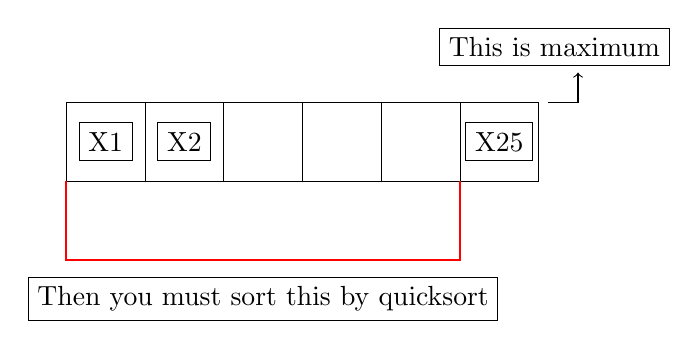
\begin{tikzpicture}
\draw[step=1cm,black,very thin] (0,0) grid (6,1)  node[anchor=north west] {};
\node[draw] at (0.5,0.5) {X1};
\node[draw] at (1.5,0.5) {X2};
\node[draw] at (5.5,0.5) {X25};
\node[draw] at (6.2,1.7) {This is maximum};
\node[draw] at (2.5,-1.5) {Then you must sort this by quicksort};
\node (A) at (6, 1) {};
\node (B) at (6.5, 1.5) {};
\draw[->, to path={-| (\tikztotarget)}]
  (A) edge (B) ;
\draw[red,thick,solid] (0,0) -- (0,-1) -- (5,-1) -- (5,0);
\end{tikzpicture} 
Minimum, \\ 
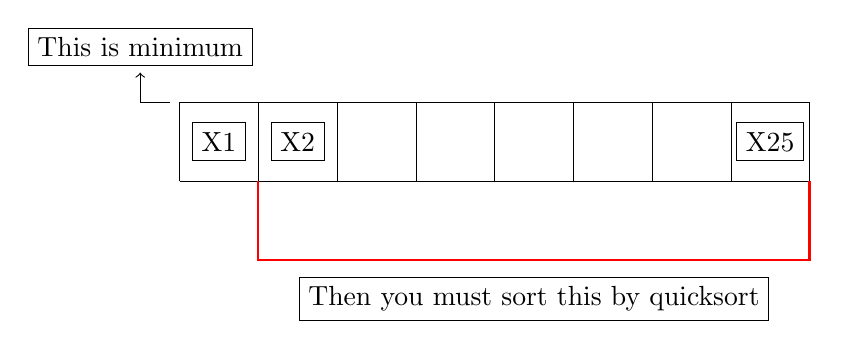
\begin{tikzpicture}
\draw[step=1cm,black,very thin] (0,0) grid (8,1)  node[anchor=north west] {};
\node[draw] at (0.5,0.5) {X1};
\node[draw] at (1.5,0.5) {X2};
\node[draw] at (7.5,0.5) {X25};
\node[draw] at (-0.5,1.7) {This is minimum};
\node[draw] at (4.5,-1.5) {Then you must sort this by quicksort};
\node (A) at (0, 1) {};
\node (B) at (-0.5, 1.5) {};
\draw[->, to path={-| (\tikztotarget)}]
  (A) edge (B) ;
\draw[red,thick,solid] (1,0) -- (1,-1) -- (8,-1) -- (8,0);
\end{tikzpicture}
